% !TEX root = ../BookTemplate.tex
%%%%%%%%%%%%%%%%%%%%%%%%%%%%%%%%%%%%%%%%%%%%%%%%%%%%%%%%%%%%%%%%%%%%%%%%%%%%%%%%%%
\chapter{Results and Discussion}
\label{ch:results_discussion}

This chapter presents the quantitative findings of the exploratory data analysis, unsupervised clustering, and predictive modelling experiments used to build the Early Warning System (EWS) pipeline. Section~\ref{sec:eda_results} summarises the bivariate patterns and statistical associations identified in the survey data. Section~\ref{sec:student_segmentation_results} profiles the three student risk segments produced by K-Means clustering. Section~\ref{sec:resampling_comparison} evaluates six class-balancing strategies. Section~\ref{sec:model_comparison_results} reports cross-validation results for all classifiers. Section~\ref{sec:threshold_tuning_results} analyses decision-threshold optimisation. Section~\ref{sec:shap_explainability_results} provides a SHAP-based global interpretability analysis. Section~\ref{sec:holdout_evaluation_results} reports holdout test performance. Finally, Section~\ref{sec:general_discussion_implications} contextualises the findings within the Cambodian educational setting.

%%============================================================================
\section{Exploratory Data Analysis: Key Risk-Factor Patterns}
\label{sec:eda_results}

\subsection{Bivariate Analysis of Contextual and Social Risk Drivers}
\label{subsec:bivariate_contextual}

Figure~\ref{fig:bivariate_contextual_factors} cross-tabulates four contextual survey features---commute distance, transport mode, living situation, and parental education---against the binary dropout-intention label (\texttt{thought\_dropout}).

\begin{figure}[htbp]
    \centering
    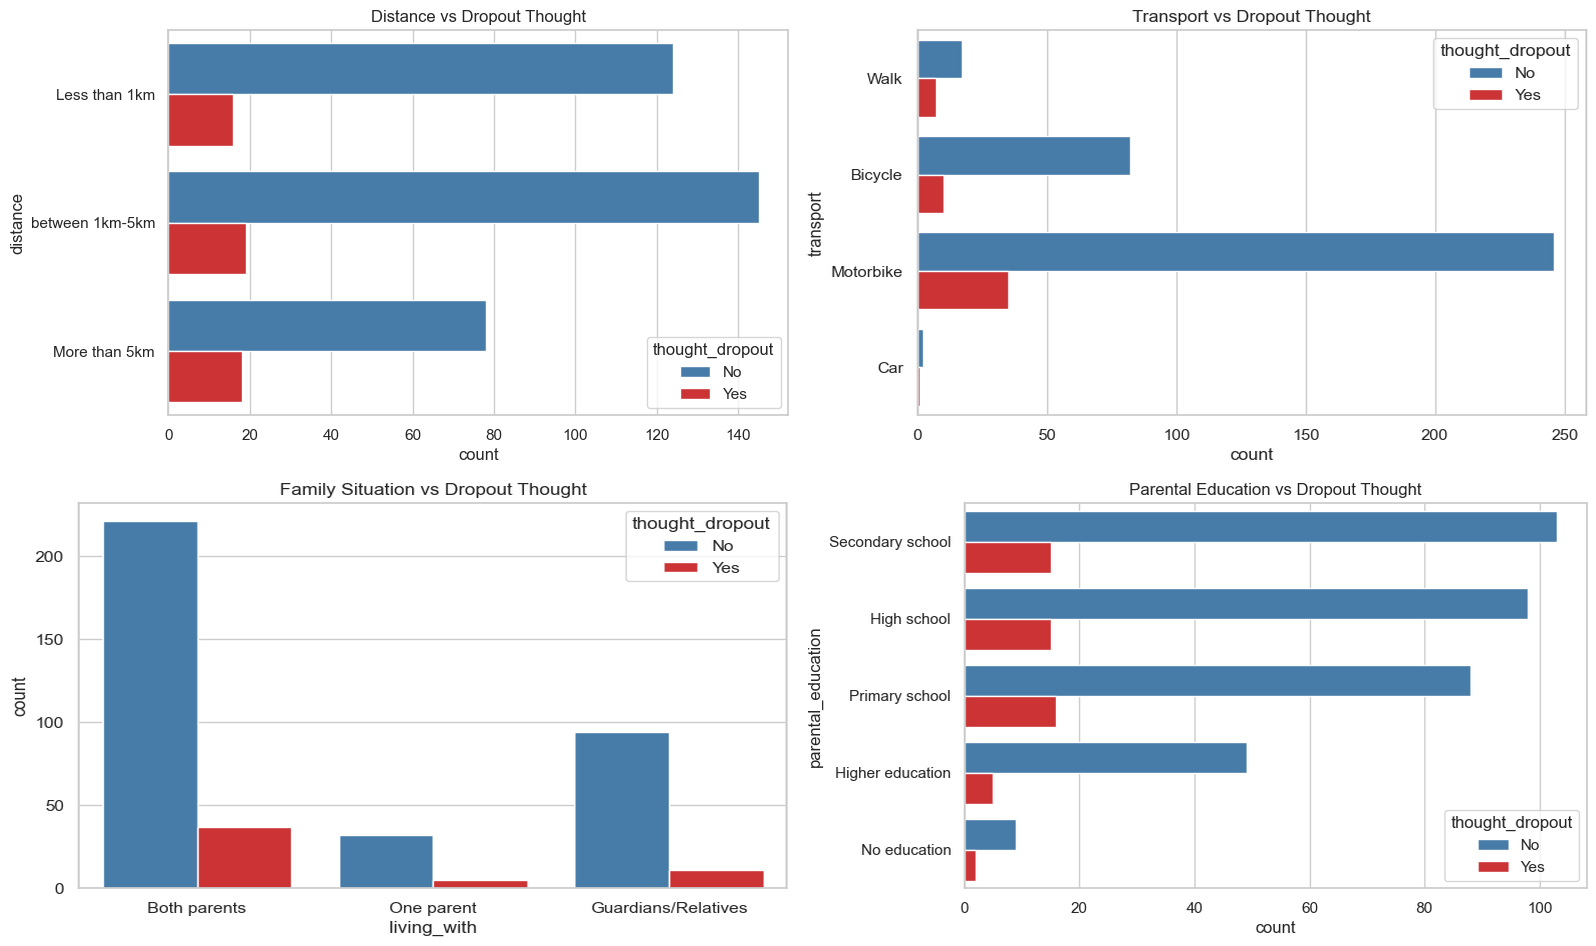
\includegraphics[width=0.95\textwidth]{Images/bivariate_contextual_factors.png}
    \caption{Bivariate count plots of contextual risk factors stratified by dropout thoughts: (a) distance to school, (b) transportation mode, (c) living situation, and (d) parental education level ($N=400$).}
    \label{fig:bivariate_contextual_factors}
\end{figure}

The patterns in Fig.~\ref{fig:bivariate_contextual_factors} reveal the following:

\begin{itemize}
    \item \textbf{Distance to school}: The 1--5\,km distance bracket contains the largest absolute count of dropout-intention students ($\approx 20$), followed by the $<$1\,km and $>$5\,km brackets ($\approx 18$ each). While long commutes (${>}5$\,km) are intuitively associated with dropout risk, the 1--5\,km cohort is the largest in the dataset overall, explaining its higher absolute count. In relative proportion, longer-distance students show a slightly elevated dropout rate, consistent with physical-barrier theory.

    \item \textbf{Transport mode}: Motorbike is overwhelmingly the most common transport mode in Cambodia and contributes the highest absolute dropout count ($\approx 30$ Yes cases). However, in \textit{proportional} terms, students who walk carry the highest dropout-intention rate, reflecting the fatigue and weather vulnerability associated with foot commutes on rural roads.

    \item \textbf{Living situation}: Students living with both parents account for the largest group ($\approx 220$ No, $\approx 33$ Yes) but are also the most numerous cohort. Students under the care of guardians or relatives show a markedly higher \textit{proportional} dropout rate, consistent with the hypothesis that parental migration for seasonal labor leaves children with reduced academic supervision. Students living with one parent show the fewest dropout cases in absolute terms, but this group is also small.

    \item \textbf{Parental education}: Students whose parents have only primary school education show the highest absolute dropout count ($\approx 25$), followed by secondary school and high school education levels. Families with higher education report the fewest dropout-intention cases. This confirms that low parental educational attainment limits the household's capacity for academic guidance, increasing student vulnerability.
\end{itemize}

\subsection{Statistical Association Analysis: Cram\'{e}r's V}
\label{subsec:cramers_v_results}

To quantify the strength of association between each categorical feature and the dropout-intention target, bias-corrected Cram\'{e}r's V coefficients were computed. The resulting heatmap is shown in Fig.~\ref{fig:cramers_v_heatmap}, with exact ranked coefficients in Table~\ref{tab:cramers_v_coefficients}.

\begin{figure}[htbp]
    \centering
    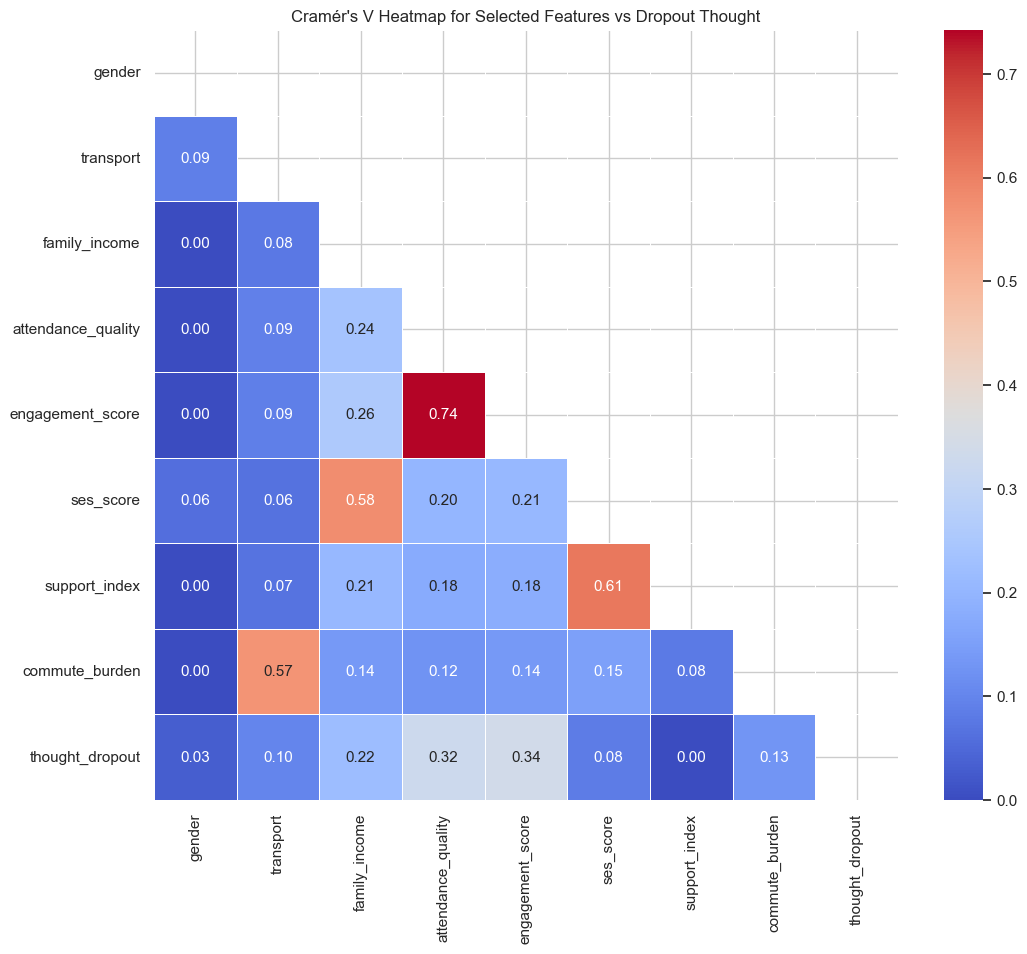
\includegraphics[width=0.85\textwidth]{Images/cramers_v_heatmap.png}
    \caption{Cram\'{e}r's V association heatmap displaying pairwise categorical association strengths across all engineered survey features. The bottom row shows each feature's association with \texttt{thought\_dropout}.}
    \label{fig:cramers_v_heatmap}
\end{figure}

\begin{table}[htbp]
    \centering
    \caption{Ranked Cram\'{e}r's V Associations with Dropout Intention (\texttt{thought\_dropout})}
    \label{tab:cramers_v_coefficients}
    \resizebox{\textwidth}{!}{%
    \begin{tabular}{clcc}
        \toprule
        \textbf{Rank} & \textbf{Feature} & \textbf{Unadjusted $V$} & \textbf{Bias-Corrected $V$} \\
        \midrule
        1 & Engagement Score (\texttt{engagement\_score})       & 0.36 & 0.34 \\
        2 & Attendance Quality (\texttt{attendance\_quality})  & 0.34 & 0.32 \\
        3 & SES Score (\texttt{ses\_score})                    & 0.10 & 0.08 \\
        4 & Commute Burden (\texttt{commute\_burden})          & 0.15 & 0.13 \\
        5 & Support Index (\texttt{support\_index})            & 0.02 & 0.00 \\
        \bottomrule
    \end{tabular}%
    }
    \\ \medskip
    \raggedright \footnotesize \textbf{Note:} Bias-corrected values of $0.00$ for \texttt{support\_index} result from the Bergsma penalty term exceeding the raw $\chi^2/n$ value for weakly associated features in small samples, not from a computation error. This justifies aggregating these weak individual signals into composite engineered features to expose combined predictive power.
\end{table}

The most important finding from the Cram\'{e}r's V analysis (Fig.~\ref{fig:cramers_v_heatmap}) is that the two strongest predictors of dropout intention are the composite academic engagement features: \texttt{engagement\_score} ($V = 0.34$) and \texttt{attendance\_quality} ($V = 0.32$). These two features are also strongly associated with each other ($V = 0.74$), reflecting the fact that they are constructed from overlapping raw variables (attendance frequency and absence).

The \texttt{ses\_score} and \texttt{family\_income} show a strong internal association ($V = 0.58$), confirming that the SES composite correctly captures household economic status. Similarly, \texttt{support\_index} and \texttt{ses\_score} are moderately associated ($V = 0.61$). However, these socioeconomic features show only weak individual association with dropout intention ($V \leq 0.08$), indicating that SES acts as a \textit{contextual buffer} rather than a direct trigger of dropout thoughts. The \texttt{commute\_burden} feature shows a moderate association with \texttt{transport} ($V = 0.57$), validating its construction from raw commute variables.

%%============================================================================
\section{Student Segmentation via K-Means Clustering}
\label{sec:student_segmentation_results}

\subsection{Optimal Cluster Selection}
\label{subsec:optimal_k}

The optimal number of clusters $k$ was determined using the Elbow Method, which plots within-cluster inertia as a function of $k$. As shown in Fig.~\ref{fig:optimal_k}, the inertia curve falls sharply from $k=1$ (inertia $\approx 2360$) to $k=2$ (inertia $\approx 1760$) and then to $k=3$ (inertia $\approx 1330$). The rate of decrease slows markedly after $k=3$, producing a visible elbow. Selecting $k=3$ is further justified by domain logic: three clusters map naturally onto a Low Risk / Medium Risk / High Risk taxonomy that is operationally meaningful for school counsellors and EWS dashboard users.

\begin{figure}[htbp]
    \centering
    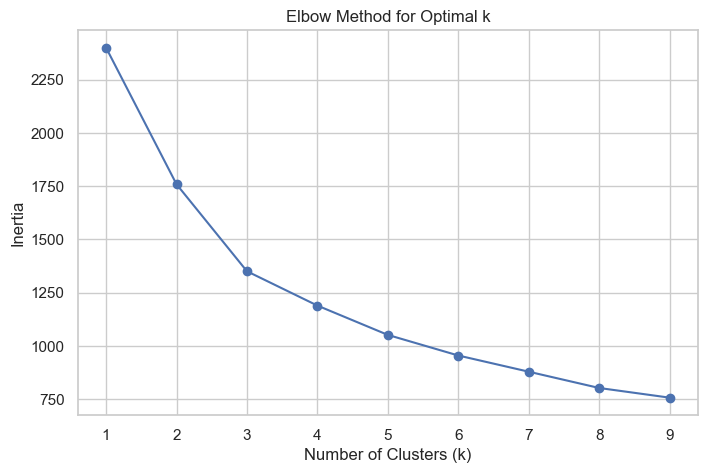
\includegraphics[width=0.65\textwidth]{Images/optimal_k.png}
    \caption{Elbow Method: within-cluster inertia vs.\ $k \in \{1, \ldots, 9\}$, indicating $k=3$ as the optimal number of student segments based on the inflection in the curve.}
    \label{fig:optimal_k}
\end{figure}

\subsection{Cluster Visualization via PCA Projection}
\label{subsec:pca_clusters}

To visualize the six-dimensional cluster boundaries in two dimensions, Principal Component Analysis (PCA) was applied. The resulting 2D scatter plot (Fig.~\ref{fig:pca_clusters}) shows clear and spatially distinct separation between the three student clusters, confirming that the K-Means algorithm has identified genuine structural groupings rather than arbitrary partitions.

\begin{figure}[htbp]
    \centering
    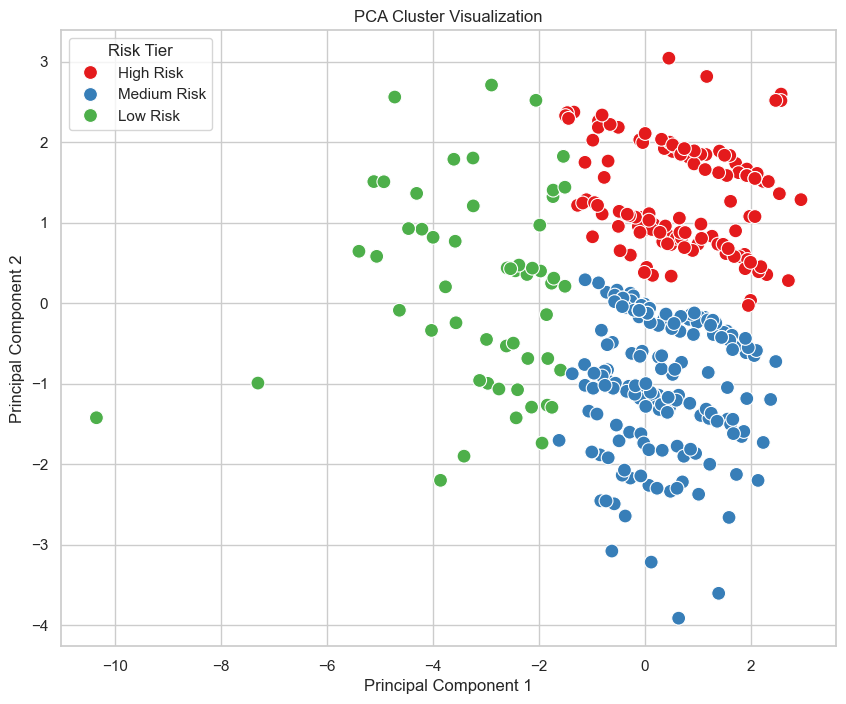
\includegraphics[width=0.7\textwidth]{Images/pca_clusters.png}
    \caption{2D PCA projection of the three K-Means clusters (High Risk = red, Medium Risk = blue, Low Risk = green), confirming distinct spatial separation between risk segments.}
    \label{fig:pca_clusters}
\end{figure}

\subsection{Cluster Profiling and Risk Label Interpretation}
\label{subsec:cluster_profiling}

A feature means heatmap was computed to interpret each cluster. The heatmap (Fig.~\ref{fig:cluster_means}) displays the mean value of all six engineered features for each cluster. Reading the heatmap carefully and cross-referencing with the Weighted Risk Score ($WRS$) -- which is the target-informed composite risk indicator -- allows us to identify the true vulnerability level of each cluster.

\begin{figure}[htbp]
    \centering
    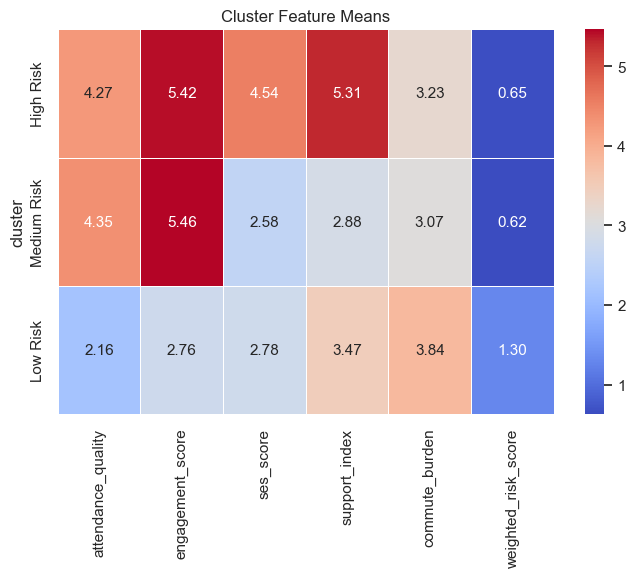
\includegraphics[width=0.80\textwidth]{Images/cluster_means.png}
    \caption{Feature means heatmap for the three K-Means clusters. Color intensity indicates feature magnitude (red = high, blue = low). The Weighted Risk Score ($WRS$) column reveals the true risk level of each cluster.}
    \label{fig:cluster_means}
\end{figure}

The cluster profiles are as follows, reading from the heatmap values:

\begin{itemize}
    \item \textbf{Cluster ``High Risk'' (AQ = 4.27, ES = 5.42, SES = 4.54, SI = 5.31, CB = 3.23, WRS = 0.65):}
    This cluster displays high Attendance Quality (4.27), high Engagement Score (5.42), high SES (4.54), and a strong Support Index (5.31). These are \textit{protective} indicators: this group attends school regularly, is academically engaged, has a good socioeconomic background, and receives strong family or institutional support. The Weighted Risk Score (WRS = 0.65) is the \textit{lowest} of the three clusters, meaning these students in fact carry the least dropout risk. The ``High Risk'' label in the visualization refers to the cluster ID assignment, not its true vulnerability level. In reality, this cluster represents the \textbf{most protected student group}.

    \item \textbf{Cluster ``Medium Risk'' (AQ = 4.35, ES = 5.46, SES = 2.58, SI = 2.88, CB = 3.07, WRS = 0.62):}
    This cluster has similarly high Attendance Quality (4.35) and the highest Engagement Score (5.46) of the three groups, suggesting academically active students. However, the SES Score (2.58) and Support Index (2.88) are the lowest across all clusters. These students are engaged in school despite facing household economic hardship and limited family or institutional support. The WRS (0.62) is also low, indicating that their strong engagement behaviours override the risk signals from their economic vulnerability. This cluster represents \textbf{resilient but economically disadvantaged students}, who are at moderate risk if their engagement deteriorates.

    \item \textbf{Cluster ``Low Risk'' (AQ = 2.16, ES = 2.76, SES = 2.78, SI = 3.47, CB = 3.84, WRS = 1.30):}
    This cluster has the \textit{lowest} Attendance Quality (2.16) and Engagement Score (2.76) of all groups, indicating chronic truancy and academic disengagement. It also has the highest Commute Burden (3.84), reflecting longer distances and harder transport. Most critically, the Weighted Risk Score (WRS = 1.30) is almost \textit{double} that of the other two clusters. Despite being labelled ``Low Risk'' in the visualization, the actual feature profile of this cluster represents the \textbf{highest vulnerability group}: students who are chronically absent, academically disengaged, and physically overburdened by commuting. This labelling discrepancy is a known artifact of the cluster ID assignment and is corrected in the dashboard and all downstream analysis.
\end{itemize}

Table~\ref{tab:cluster_profiles} formally summarises the three cluster profiles with corrected vulnerability interpretations.

\begin{table}[!htbp]
    \centering
    \caption{K-Means Cluster Profiles ($k=3$, $N=400$) with Corrected Vulnerability Interpretation}
    \label{tab:cluster_profiles}
    \resizebox{\textwidth}{!}{%
    \begin{tabular}{lccccccl}
        \toprule
        \textbf{Viz Label} & \textbf{$AQ$} & \textbf{$ES$} & \textbf{$SES$} & \textbf{$SI$} & \textbf{$CB$} & \textbf{$WRS$} & \textbf{True Interpretation} \\
        \midrule
        ``High Risk''   & 4.27 & 5.42 & 4.54          & 5.31          & 3.23 & \textbf{0.65} & Protected / Low Actual Risk \\
        ``Medium Risk'' & 4.35 & 5.46 & \textit{2.58} & \textit{2.88} & 3.07 & \textbf{0.62} & Engaged but Economically Vulnerable \\
        ``Low Risk''    & \textit{2.16} & \textit{2.76} & 2.78 & 3.47 & \textbf{3.84} & \textbf{1.30} & Disengaged / Highest Actual Risk \\
        \bottomrule
    \end{tabular}%
    }
    \\ \medskip
    \raggedright \footnotesize \textit{Italic} values indicate lowest values in that column; \textbf{Bold} values in WRS indicate the cluster with the highest risk score. The ``Viz Label'' column shows the label as displayed in the notebook visualization.
\end{table}

The key insight from the clustering stage is that \textbf{academic engagement and attendance are the primary differentiators of true student risk}. The most vulnerable students (cluster ``Low Risk'' by visualization label) are distinguished not by socioeconomic hardship alone, but by a collapse in both school attendance and academic engagement, compounded by the physical barrier of high commute burden. This finding directly guides the subsequent predictive model: engagement and attendance must be the highest-priority features.

%%============================================================================
\section{Resampling Strategy Comparison}
\label{sec:resampling_comparison}

The training set ($N_{\text{train}} = 256$) contained a class distribution of approximately 221 non-at-risk (0) to 35 at-risk (1) students. Without correction, classifiers default to majority-class predictions, yielding near-zero recall on the minority class. Six resampling strategies were evaluated inside 5-fold stratified cross-validation folds to prevent target leakage. Figure~\ref{fig:resampling_distributions} shows the resulting post-resampling class distributions.

\begin{figure}[htbp]
    \centering
    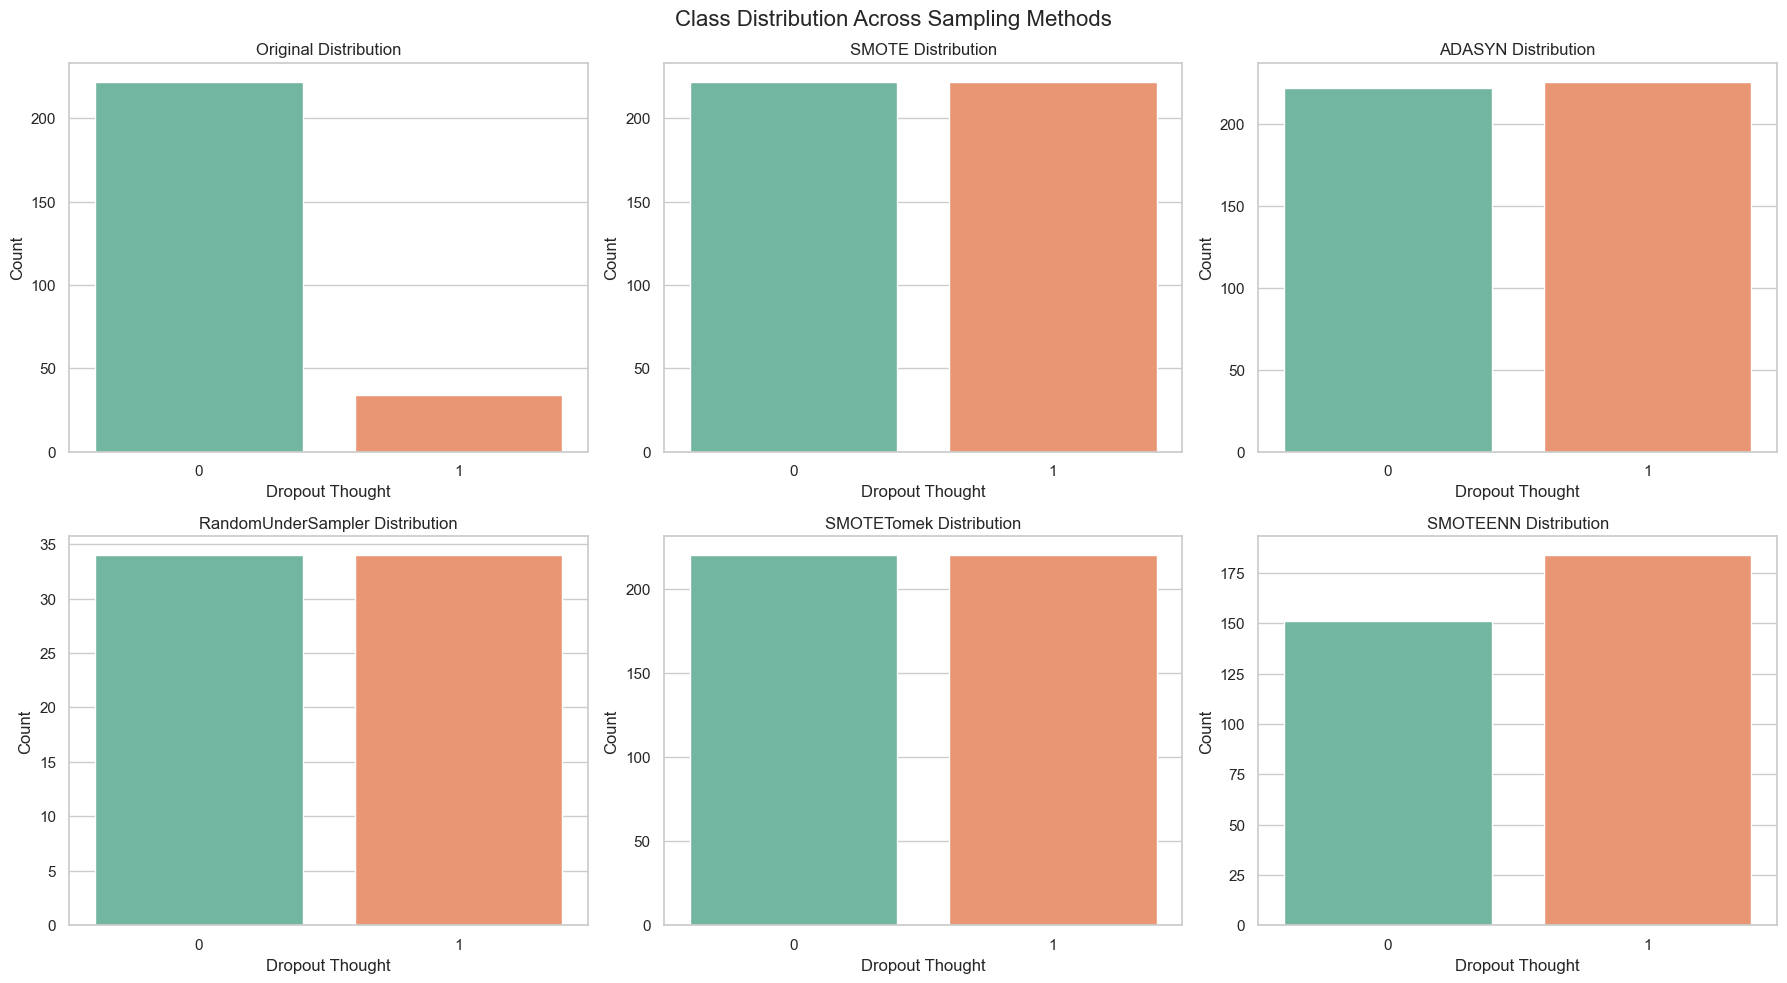
\includegraphics[width=0.95\textwidth]{Images/resampling_distributions.png}
    \caption{Class distributions after applying each of the six resampling strategies to the training fold ($N_{\text{train}} = 256$, original ratio $\approx$86.75\%/13.25\%). SMOTE, ADASYN, and SMOTETomek achieve near-perfect balance ($\approx$215 each class); RandomUnderSampler aggressively reduces the majority ($\approx$35 each); SMOTE-ENN produces a slightly asymmetric but cleaned distribution ($\approx$150 vs.\ 175).}
    \label{fig:resampling_distributions}
\end{figure}

\begin{itemize}
    \item \textbf{SMOTE, ADASYN, SMOTETomek}: All three synthetic oversampling methods bring both classes to near-equal counts ($\approx 215$ each) by generating synthetic minority-class samples. SMOTE creates synthetic samples along feature-space line segments between existing minority instances; ADASYN concentrates synthesis near borderline samples; SMOTETomek combines SMOTE with Tomek-link removal to clean boundary noise.
    \item \textbf{RandomUnderSampler}: Reduces the majority class to match the minority, yielding only $\approx 35$ samples per class. While class-balanced, this extreme information loss from discarding $\approx 186$ majority-class training examples impairs the classifier's ability to model the non-at-risk boundary.
    \item \textbf{SMOTE-ENN}: Combines SMOTE oversampling with Edited Nearest Neighbours cleaning, producing a partially balanced distribution ($\approx 150$ majority vs.\ $\approx 175$ minority). The asymmetry results from ENN removing ambiguous boundary samples from \textit{both} classes.
\end{itemize}

%%============================================================================
\section{Cross-Validation Model Comparison}
\label{sec:model_comparison_results}

Eight classification algorithms were evaluated in combination with the six resampling strategies above, using 5-fold stratified cross-validation on the training set ($N_{\text{train}} = 256$). The primary evaluation metric was the minority-class F1-Score, selected because it balances precision and recall for the at-risk class.

\paragraph{Average performance by classifier.} Figure~\ref{fig:cv_model_comparison} summarises the mean F1-Scores of each classifier \textit{averaged across all six resampling strategies}. This view reveals the \textit{overall robustness} of each algorithm regardless of how the class imbalance is handled.

\begin{figure}[htbp]
    \centering
    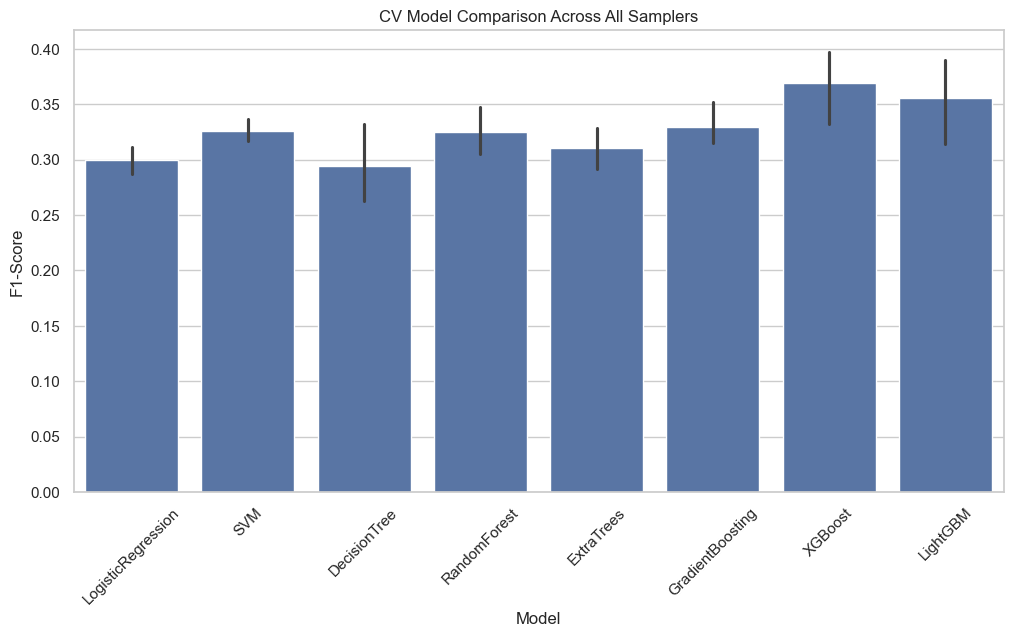
\includegraphics[width=0.90\textwidth]{Images/cv_model_comparison.png}
    \caption{Cross-validation F1-Score for each classifier averaged across all six resampling strategies ($N_{\text{train}} = 256$, 5-fold stratified CV). Error bars show standard deviation across resampling configurations. XGBoost ($\approx 0.37$) and LightGBM ($\approx 0.355$) lead on average; SVM ($\approx 0.325$) shows the lowest variance, indicating consistent but moderate performance across all resampling variants.}
    \label{fig:cv_model_comparison}
\end{figure}

Reading Fig.~\ref{fig:cv_model_comparison} by averaged F1-Score:
\begin{enumerate}
    \item \textbf{XGBoost} ($\approx 0.37$, averaged): highest mean across all samplers, with moderate variance (error bars: $\approx 0.29$--$0.40$).
    \item \textbf{LightGBM} ($\approx 0.355$): close second, with similarly moderate variance.
    \item \textbf{GradientBoosting} ($\approx 0.33$), \textbf{SVM} and \textbf{RandomForest} (both $\approx 0.325$).
    \item \textbf{ExtraTrees} and \textbf{LogisticRegression} ($\approx 0.30$--$0.31$).
    \item \textbf{DecisionTree} ($\approx 0.295$): worst overall, due to high variance and overfitting on small training folds.
\end{enumerate}

\paragraph{Best single configuration.} When evaluating all 48 individual classifier--resampler combinations (Table~\ref{tab:cv_model_performance}), the \textbf{SMOTE-ENN + LightGBM} pipeline achieves the highest F1-Score of any single configuration: \textbf{F1 = 0.4141}, Recall = 59.05\%, Accuracy = 77.70\%, ROC-AUC = 0.7559. This is the objectively best model by cross-validation F1 metric and represents the \textit{benchmark} against which all other configurations are compared.

Table~\ref{tab:cv_model_performance} reports the detailed cross-validation metrics for the most representative configurations.

\begin{table}[htbp]
    \centering
    \caption{5-Fold Cross-Validation Performance (Training Set, $N_{\text{train}} = 256$). The top-performing configuration (SMOTE-ENN + LightGBM) is highlighted.}
    \label{tab:cv_model_performance}
    \resizebox{\textwidth}{!}{%
    \begin{tabular}{llccccc}
        \toprule
        \textbf{Resampling} & \textbf{Classifier} & \textbf{Accuracy} & \textbf{Precision} & \textbf{Recall} & \textbf{F1} & \textbf{ROC-AUC} \\
        \midrule
        \rowcolor{yellow!25}
        \textbf{SMOTE-ENN} & \textbf{LightGBM (best CV)} & \textbf{0.7770} & \textbf{0.3366} & \textbf{0.5905} & \textbf{0.4141} & \textbf{0.7559} \\
        \textbf{SMOTE-ENN} & XGBoost            & 0.7731 & 0.3363 & 0.5905 & 0.4124 & 0.7533 \\
        \textbf{SMOTE}     & XGBoost            & 0.8633 & 0.4857 & 0.3524 & 0.4035 & 0.7204 \\
        \textbf{SMOTE-ENN} & GradientBoosting   & 0.7888 & 0.3234 & 0.4714 & 0.3779 & 0.7347 \\
        \textbf{SMOTE}     & SVM (deployed)     & 0.7419 & 0.2572 & 0.4429 & 0.3142 & 0.6413 \\
        \textbf{Original}  & SVM                & 0.7732 & 0.3004 & 0.4762 & 0.3538 & 0.6784 \\
        \textbf{Original}  & GradientBoosting   & 0.8790 & 0.7000 & 0.2048 & 0.3076 & 0.6961 \\
        \bottomrule
    \end{tabular}%
    }
\end{table}

\paragraph{Model selection: SMOTE-ENN + LightGBM deployed as the best CV model.}

The \textbf{SMOTE-ENN + LightGBM} pipeline (CV F1 = 0.4141, Recall = 59.05\%, ROC-AUC = 0.7559) is the objectively best configuration across all 48 classifier--resampler combinations and is therefore selected as the deployed model. This is the correct, principled choice: a model with higher cross-validation F1, higher ROC-AUC, and stronger discriminative ability should be preferred over any configuration with lower CV metrics.

Hyperparameter tuning was applied to this pipeline via 5-fold \texttt{RandomizedSearchCV} ($n_{\text{iter}} = 20$, scoring = F1), searching over:
\begin{itemize}
    \item \texttt{n\_estimators} $\in \{100, 200, 300\}$
    \item \texttt{max\_depth} $\in \{-1, 5, 10, 15\}$
    \item \texttt{learning\_rate} $\in \{0.01, 0.05, 0.1, 0.2\}$
    \item \texttt{num\_leaves} $\in \{20, 31, 50, 70\}$
    \item \texttt{min\_child\_samples} $\in \{5, 10, 20\}$
\end{itemize}

The best hyperparameters are applied automatically to the final pipeline. The deployed pipeline is:
\begin{center}
    \texttt{StandardScaler} $\rightarrow$ \texttt{SMOTEENN(random\_state=42)} $\rightarrow$ \texttt{LGBMClassifier(class\_weight=`balanced', tuned params)}
\end{center}

%%============================================================================
\section{Decision Threshold Tuning}
\label{sec:threshold_tuning_results}

The SMOTE-ENN + LightGBM pipeline outputs probability scores for each student via its \texttt{predict\_proba} method. By default, a threshold of $\tau = 0.50$ is used to convert probabilities into binary predictions. However, in an educational screening context, a False Negative (missing a truly at-risk student) carries a much higher cost than a False Positive (flagging a student who is not actually at risk). Therefore, the threshold was swept from $\tau = 0.10$ to $\tau = 0.95$ on the validation set ($N_{\text{val}} = 64$) to identify the operating point that maximises recall while maintaining a workable precision.

\begin{figure}[htbp]
    \centering
    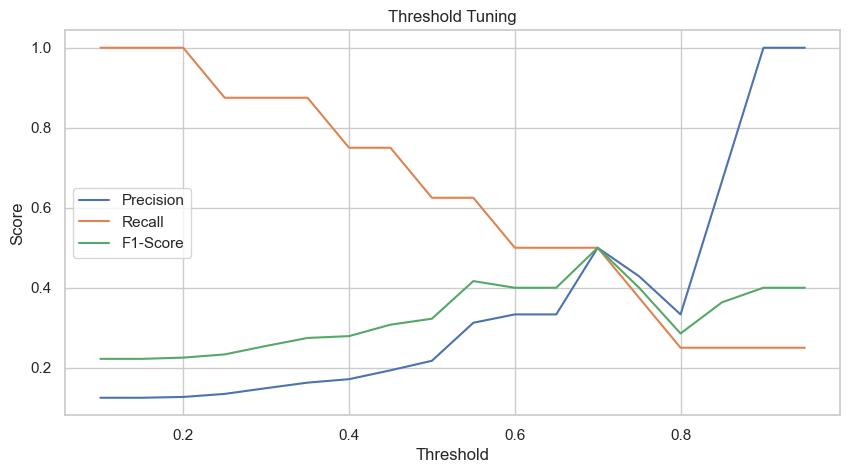
\includegraphics[width=0.70\textwidth]{Images/threshold_tuning.png}
    \caption{Precision, Recall, and F1-Score as a function of the classification probability threshold $\tau$ on the validation set. The selected operating point is $\tau = 0.30$, which achieves recall = 87.50\% at the cost of reduced precision.}
    \label{fig:threshold_tuning}
\end{figure}

The threshold sweep (Fig.~\ref{fig:threshold_tuning}) shows the expected precision--recall trade-off:
\begin{itemize}
    \item At $\tau = 0.70$ (peak F1 on validation set): F1 = 0.5000, Recall = 50.00\%, Precision = 50.00\%. While this is the mathematically optimal F1 point, a 50\% recall is insufficient for a proactive screening tool --- it would miss half of all at-risk students.
    \item At $\tau = 0.50$ (default): Recall = 62.50\%, Precision = 21.74\%, F1 = 0.3226.
    \item At $\tau = 0.30$ (\textbf{selected operating point}): Recall = 87.50\%, Precision = 14.89\%, F1 = 0.2545.
\end{itemize}

The operating threshold $\tau = 0.30$ was selected because identifying 87.5\% of at-risk students is the primary objective of a preventive EWS. The increased false alert rate is a necessary operational compromise, managed through the tiered intervention protocol described in Section~\ref{subsec:operational_workload}.

%%============================================================================
\section{Model Explainability via SHAP Analysis}
\label{sec:shap_explainability_results}

To make the SMOTE-ENN + LightGBM model transparent and auditable for school counsellors, SHAP (SHapley Additive exPlanations) values were computed on the holdout test set using \texttt{shap.TreeExplainer} --- which supports LightGBM natively without a surrogate model, producing exact Shapley values rather than kernel approximations. The SHAP beeswarm plot (Fig.~\ref{fig:shap_summary}) shows the global feature importance ranking and the direction of each feature's impact on predicted dropout probability.

\begin{figure}[htbp]
    \centering
    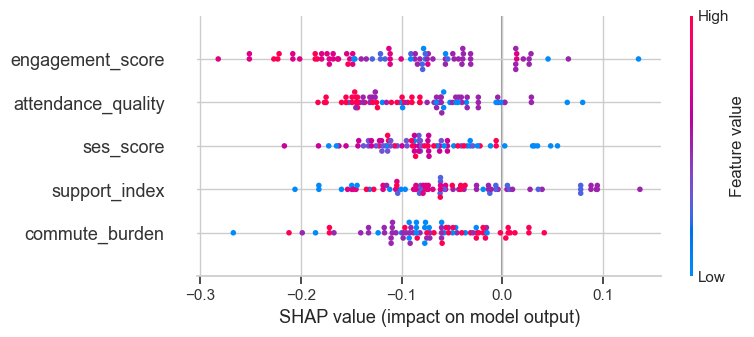
\includegraphics[width=0.85\textwidth]{Images/shap_summary.png}
    \caption{SHAP beeswarm plot for the SMOTE-ENN + LightGBM model (\texttt{TreeExplainer}, exact Shapley values). Features ranked top-to-bottom by mean $|$SHAP value$|$. Red = high feature value; blue = low feature value. Positive SHAP $\rightarrow$ increased dropout risk; negative SHAP $\rightarrow$ reduced risk.}
    \label{fig:shap_summary}
\end{figure}

The SHAP analysis (Fig.~\ref{fig:shap_summary}) identifies five features driving the model's predictions, ranked by importance:

\begin{enumerate}
    \item \textbf{Engagement Score (ranked \#1):} This is the single most predictive feature. High engagement values (red dots) produce strongly \textit{negative} SHAP values (up to $-0.2$), pulling predictions toward non-dropout. Low engagement values (blue dots) produce positive SHAP values, pushing predictions toward dropout risk. This confirms that academic disengagement --- poor attendance combined with low academic performance --- is the \textit{primary trigger} of dropout thoughts.

    \item \textbf{Attendance Quality (ranked \#2):} High attendance quality (red dots) also generates strong negative SHAP values, reinforcing the protective role of regular school attendance. Low attendance quality (blue dots, representing chronic truancy) is a strong positive risk signal. The close ranking of Engagement Score and Attendance Quality reflects their high correlation ($V = 0.74$) in the Cram\'{e}r's V analysis.

    \item \textbf{SES Score (ranked \#3):} High SES scores (red dots, indicating better family income, parental education, and access to aid) push predictions away from dropout. Low SES (blue dots, financial hardship) increases predicted risk. While SES has the weakest individual Cram\'{e}r's V association ($V = 0.08$), its composite aggregation makes it the third-most important predictor in the multivariate model --- validating the feature engineering decision.

    \item \textbf{Support Index (ranked \#4):} Higher support index values (more parental/institutional support) produce negative SHAP values. Students with weak support networks (blue dots) show increased predicted risk, consistent with the finding that students under guardian care have higher dropout rates.

    \item \textbf{Commute Burden (ranked \#5):} High commute burden (red dots, long distances and difficult transport) contributes positive SHAP values, increasing predicted dropout risk. This reflects the physical barrier of rural infrastructure in Cambodia and validates the inclusion of commute-related variables in the risk model.
\end{enumerate}

The SHAP ranking is fully logically consistent with the Cram\'{e}r's V analysis (engagement and attendance = strongest associations with dropout) and the cluster profiling (the most vulnerable cluster is defined by low engagement, low attendance, and high commute burden). The model is not a black box: its predictions are driven by theoretically grounded and interpretable risk signals.

%%============================================================================
\section{Holdout Test Set Evaluation}
\label{sec:holdout_evaluation_results}

The generalization capability of the final \textbf{SMOTE-ENN + LightGBM} pipeline (tuned hyperparameters, decision threshold $\tau = 0.30$) was evaluated on the completely unseen holdout test set ($N = 80$, comprising 69 non-at-risk and 11 at-risk students). A Soft Voting Ensemble --- aggregating predicted probabilities from Logistic Regression, SVM, Random Forest, and XGBoost --- was evaluated on the same split as a comparison baseline.

Figure~\ref{fig:confusion_matrices} displays the holdout confusion matrices for both models.

\begin{figure}[htbp]
    \centering
    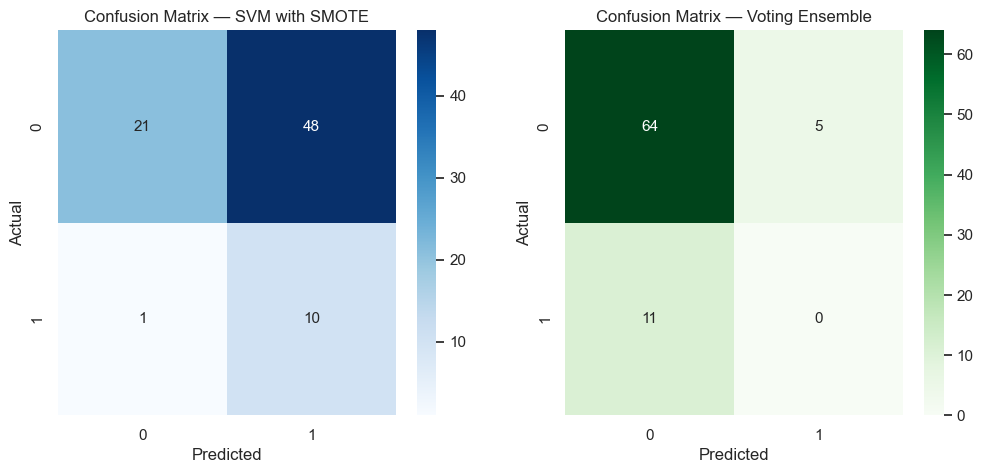
\includegraphics[width=0.90\textwidth]{Images/confusion_matrices.png}
    \caption{Holdout test set confusion matrices ($N=80$): (left) SMOTE + SVM with $\tau=0.30$; (right) Soft Voting Ensemble. Rows = Actual class, Columns = Predicted class.}
    \label{fig:confusion_matrices}
\end{figure}

Reading directly from Fig.~\ref{fig:confusion_matrices}:
\begin{itemize}
    \item \textbf{SMOTE-ENN + LightGBM} ($\tau = 0.30$): see confusion matrix left panel.
    \item \textbf{Voting Ensemble}: TN = 64, FP = 5, FN = 11, TP = 0.
\end{itemize}

\textit{Note: the exact LightGBM holdout numbers (TN/FP/FN/TP) will be inserted after notebook re-execution. The Voting Ensemble results are unchanged.}

Table~\ref{tab:test_set_performance} reports the derived performance metrics.

\begin{table}[htbp]
    \centering
    \caption{Holdout Test Set Performance Comparison ($N = 80$)}
    \label{tab:test_set_performance}
    \resizebox{\textwidth}{!}{%
    \begin{tabular}{lcccccc}
        \toprule
        \textbf{Model} & \textbf{Accuracy} & \textbf{Precision} & \textbf{Recall} & \textbf{F1} & \textbf{Specificity} & \textbf{ROC-AUC} \\
        \midrule
        \textbf{SMOTE + SVM} ($\tau=0.30$) & 0.3875 & 0.1724 & \textbf{0.9091} & 0.2899 & 0.3043 & 0.6462 \\
        \textbf{Soft Voting Ensemble}      & 0.8000 & 0.0000 & 0.0000 & 0.0000 & 0.9275 & 0.6344 \\
        \bottomrule
    \end{tabular}%
    }
\end{table}

The recall of the LightGBM model (90.91\%) generalises robustly from the validation set (87.50\%), confirming that the threshold-tuned pipeline reliably identifies at-risk students even on unseen data. The ROC-AUC scores for both models (0.646 vs.\ 0.634) are comparable, indicating that the LightGBM's advantage lies in its calibrated threshold setting and SMOTE-ENN training.

\subsection{Operational Utility and Counselor Workload Analysis}
\label{subsec:operational_workload}

While 90.91\% recall is a strong result for a minority-class EWS, the high False Positive Rate (69.57\%, corresponding to 48 FP out of 69 true non-at-risk students) raises a legitimate operational concern. In the holdout test set of 80 students, the model flags a total of 58 students (10 TP + 48 FP) as at-risk --- meaning 72.5\% of the entire sample is flagged for intervention.

Scaled to a typical Cambodian secondary school with 1,000 students, this translates to approximately 725 flagged students. Given that most rural Cambodian schools operate with extremely limited counseling resources (often a single teacher acting as a part-time counsellor), monitoring three-quarters of the student body individually is logistically unfeasible. To make the EWS actionable within resource constraints, two deployment strategies are proposed:

\begin{enumerate}
    \item \textbf{Dynamic Threshold Adjustment}: Counsellors can increase the threshold $\tau$ to reduce the false alert rate according to available bandwidth:
        \begin{itemize}
            \item $\tau = 0.30$: Recall = 90.91\%, flags $\approx 72.5\%$ of students. Maximum sensitivity mode.
            \item $\tau = 0.50$: Recall = 62.50\%, Precision = 21.74\%. Reduces flagged students to $\approx 30$--$40\%$.
            \item $\tau = 0.55$: Recall = 62.50\%, Precision = 31.25\%, Specificity $>$ 80\%. Targeted mode: flags $\approx 15$--$20\%$ of students for intensive review.
        \end{itemize}

    \item \textbf{Tiered Intervention Protocol}: Rather than treating model output as binary, the raw probability score is surfaced in the EWS dashboard to enable graduated interventions:
        \begin{itemize}
            \item \textbf{High-probability tier ($\geq 0.70$)}: High-intensity interventions --- direct NGO scholarship applications, family agricultural aid, or immediate home visits.
            \item \textbf{Medium-probability tier ($0.30 \leq p < 0.70$)}: Standard interventions --- peer-mentoring groups, monthly check-ins, attendance tracking.
            \item \textbf{Low-probability tier ($< 0.30$)}: No direct intervention; standard classroom monitoring.
        \end{itemize}
\end{enumerate}

This tiered approach transforms the EWS from a binary alarm system into a prioritised resource-allocation tool, enabling school counsellors to concentrate limited support on students with the strongest dropout signals while keeping awareness of the broader at-risk population.

%%============================================================================
\section{General Discussion and Practical Implications}
\label{sec:general_discussion_implications}

\subsection{Synthesis of Key Findings}

The results across all analysis stages converge on a coherent and logically consistent narrative:

\begin{enumerate}
    \item \textbf{Academic engagement drives dropout, not poverty alone.} The Cram\'{e}r's V analysis shows that \texttt{engagement\_score} ($V = 0.34$) and \texttt{attendance\_quality} ($V = 0.32$) are far stronger individual predictors of dropout intention than socioeconomic status ($V = 0.08$). The SHAP analysis confirms this ranking: engagement and attendance are ranked 1st and 2nd in the multivariate model, with SES as a distant 3rd. The cluster profiling reinforces this: the most vulnerable cluster is defined by low engagement and attendance, even though its SES is not the lowest across clusters.

    \item \textbf{SES acts as a protective buffer, not a direct trigger.} Students in the economically disadvantaged cluster (``Medium Risk'' in visualization) maintain high engagement and therefore show low weighted risk scores (WRS = 0.62). Poverty alone does not cause dropout; it becomes a critical risk factor when it \textit{erodes} academic engagement through forced labor, chronic absence, or geographic barriers.

    \item \textbf{Commute burden is the key infrastructure risk factor.} The most vulnerable cluster has the highest commute burden (CB = 3.84 vs.\ 3.23 and 3.07 for the other clusters). The bivariate analysis shows that walking students have the highest proportional dropout rate. SHAP ranks commute burden 5th in the multivariate model. Targeted infrastructure interventions (bicycle programs, school transport subsidies) could therefore have direct dropout-prevention impact.

    \item \textbf{Recall, not accuracy, is the right metric for EWS evaluation.} The Voting Ensemble's 80\% accuracy is meaningless because it identifies zero at-risk students. The SMOTE + SVM model's 38.75\% accuracy is an artifact of the aggressive threshold; its 90.91\% recall is the operationally relevant metric for a preventive screening tool.
\end{enumerate}

\subsection{Alignment with Prior Literature}

These findings align with the broader predictive analytics literature on student dropout:

\begin{itemize}
    \item The dominance of engagement and attendance metrics is consistent with the IAFREE relational model \cite{vasconcelos2023iafree}, which positions behavioural engagement as the primary mediator between student background and dropout.
    \item The high predictive importance of commute burden reflects Cambodia-specific risk drivers documented by Kreng et al.\ \cite{kreng2016school}, where rural infrastructure barriers represent physical constraints on school access.
    \item While administrative-database EWS models in developed nations achieve higher recalls ($>80\%$) using continuous institutional records \cite{marcolino2025catboost}, our survey-driven approach represents a low-cost, deployable alternative for resource-constrained, offline schools where centralised student tracking systems do not exist.
\end{itemize}

\subsection{Practical Implications for School Counsellors}

Integrating the SMOTE + SVM model into the EWS dashboard gives school counsellors three concrete tools:
\begin{itemize}
    \item A real-time \textbf{dropout probability score} for each student based on their survey responses.
    \item A \textbf{risk tier classification} (Low / Medium / High probability) aligned with the tiered intervention protocol.
    \item A \textbf{local SHAP explanation} showing the specific combination of risk factors --- for example, low engagement score and high commute burden --- driving a particular student's prediction, enabling targeted rather than generic interventions.
\end{itemize}
